% Drawing 70/01-3 -- folder 70, batch 01, archive page 17 (PDF page 18).
% Transcription: matrice par blocs de $\sigma_i$ : identité d'ordre $i-1$ en haut à gauche ; bloc $\begin{pmatrix}0&1\\1&0\end{pmatrix}$ aux places $i,i+1$, suivi sur ces deux lignes de $-(1+\alpha_i)\ \cdots\ -(1+\alpha_i)$ et $(1+\alpha_i)\ \cdots\ (1+\alpha_i)$ ; identité sur le reste de la diagonale ; dernière colonne $(0,\dots,0,1)$. Plusieurs entrées retouchées.
% Kind: block matrix of sigma_i (written out). Method 2 (schematic redraw from the facsimile). Status: partial.
% Notes: sigma_i = ( identity block (1, dots), the block (0 1 / 1 0) at places i, i+1 followed on these rows by -(1+alpha_i) ... -(1+alpha_i) and (1+alpha_i) ... (1+alpha_i); identity on the rest of the diagonal (dots, 1, 1); last column 0, ..., 0, 1; a large 0 above the right block ), inside a system brace on the left. Several entries retouched (overinked strokes on the left edge and the last column): placed as text in their positions.
% Coordinates: 1 unit = 1 mm = 1/100 of the crop width (bbox in page fractions: [0.15, 0.64, 0.92, 0.88]).
% Redrawn by Claude (claude-opus-5-5), issue #73, 2026-11-07; not checked by a human; not compiled (no TeX in the session).
% Rights: reproduces part of the work -- behind RENDER_TRANSCRIPTS, never published by itself.
\documentclass[tikz,border=3pt]{standalone}
\usepackage{amsmath,amssymb}
\usetikzlibrary{patterns,arrows.meta}
\tikzset{pencil/.style={black!45}, struck/.style={black!35}, mark/.style={circle,draw,inner sep=1.3pt}, pt/.style={circle,fill,inner sep=0.9pt}, opt/.style={circle,draw,fill=white,inner sep=1.1pt}}
\begin{document}
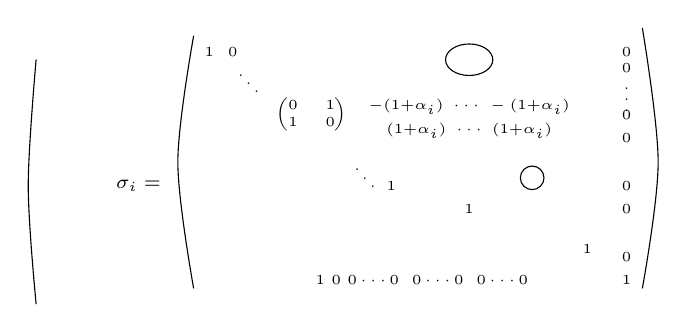
\begin{tikzpicture}[x=1mm,y=1mm,line cap=round,line join=round,font=\scriptsize]
\draw plot[smooth, tension=0.55] coordinates {(17,-9) (16,-25) (17,-40)};
\draw plot[smooth, tension=0.55] coordinates {(37,-6) (35,-22) (37,-38)};
\draw plot[smooth, tension=0.55] coordinates {(94,-5) (96,-22) (94,-38)};
\node[inner sep=1pt] at (30,-25) {\scriptsize $\sigma_i=$};
\node[inner sep=1pt] at (39,-8) {\tiny $1$};
\node[inner sep=1pt] at (42,-8) {\tiny $0$};
\node[inner sep=1pt] at (44,-11) {\tiny $\ddots$};
\node[inner sep=1pt] at (52,-16) {\tiny $\begin{pmatrix}0&1\\1&0\end{pmatrix}$};
\draw (72,-9) ellipse[x radius=3, y radius=2];
\node[inner sep=1pt] at (72,-15) {\tiny $-(1{+}\alpha_i)\ \cdots\ -(1{+}\alpha_i)$};
\node[inner sep=1pt] at (72,-18) {\tiny $(1{+}\alpha_i)\ \cdots\ (1{+}\alpha_i)$};
\node[inner sep=1pt] at (60,-23) {\tiny $\ddots\ 1$};
\node[inner sep=1pt] at (72,-28) {\tiny $1$};
\draw (80,-24) circle[radius=1.5];
\node[inner sep=1pt] at (87,-33) {\tiny $1$};
\node[inner sep=1pt] at (66,-37) {\tiny $1\ 0\ 0\cdots 0\ \ 0\cdots 0\ \ 0\cdots 0$};
\node[inner sep=1pt] at (92,-8) {\tiny $0$};
\node[inner sep=1pt] at (92,-10) {\tiny $0$};
\node[inner sep=1pt] at (92,-16) {\tiny $0$};
\node[inner sep=1pt] at (92,-19) {\tiny $0$};
\node[inner sep=1pt] at (92,-25) {\tiny $0$};
\node[inner sep=1pt] at (92,-28) {\tiny $0$};
\node[inner sep=1pt] at (92,-34) {\tiny $0$};
\node[inner sep=1pt] at (92,-13) {\tiny $\vdots$};
\node[inner sep=1pt] at (92,-37) {\tiny $1$};
\end{tikzpicture}
\end{document}
